\subsection{Single entity training}\label{ssec:SET}

We have shown that training the proposed 3D-UNet with the given training algorithm and dataloading scheme can reach very good accuracy concering the provided entity. 
It reached very high dose conformaty for single tested segments aswell as entire treatment plan dose distributions with mean gamma passrates of 94.4\% ± 6.0\% and 96.2\% ± 6.1\% respectively. 
DVH analysis, depicted in \autoref{fig:dvh}, also shows very good agreement in high dose areas, such as CTV and PTV, aswell as \acs{OAR} such as rectum or femur heads. 
Dose prediction is very accurate for the entirety of prostate plan segments with various fieldsizes, shapes, radiation angles and patient anatomies. 
The prediction was fast with inference times of 3 seconds per segment.
This is a step in the direction of online plan adaption. 
With further developement and the usage of paralleization the inference time could be further reduced. 
Nonetheless, 3 seconds is a significant improvement over 4 hours of Monte Carlo simulation time on an \acs{HPC} solution that already benefits from paralization.\\
In contrast to other previous works such as \citeauthor{kontaxis_deepdose_2020}~\cite{kontaxis_deepdose_2020}, that only included segments of five pre-defined beam angles into the training data, we did not limit us to specific beam angles but rather took the angles provided by the planning system.
We further improved on their work by increasing the voxel size in sagital and coronal directions to increase the resolution of the dose distributions and to be able to achieve higher accuracy in high density gradients. \\
Testing against entities have shown the limits of this single entity trained approach. Rapidly decreasing gamma passrates with a lowest passrate of 1.9\% for a breast cancer case were reached. 
Particularly low gamma-pass rates were obtained at tangential irradiation angles, where the radiation field passed only through the breast.
Predicted values are particularly small for these segments. An example of three poorly predicted segments is depicted in \autoref{fig:mamma}.
We assume that due to the offset of the radiation target and the associated larger distance between the target and the central beam line, the effects of the distance mask for the central beam line are overweighted and thus reduce the predicted value.

\begin{figure}
    \centering
    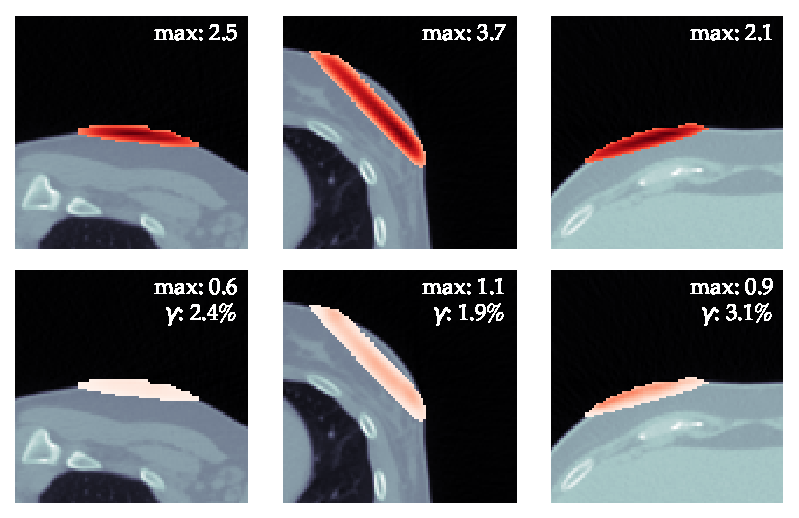
\includegraphics[width=0.9\textwidth]{mamma.pdf}
    \caption{
        Exemplary images of target dose distribution of tangential segments on breast cancer patients with very small gamma-passrates (top) and the respective dose prediction from the prostate only trained model (bottom).}\label{fig:mamma}
\end{figure}

This change in performance and accuracy is most probably occuring due to the increased complexity in testing data. 
The position of the prostate and the surrounding \acs{OAR} is quite defined inside the humans anatomy irrespective of the individual patient. 
Therefore prostate cancer treatment plans have a very similar iso center, aswell as the majority of highly contributing segments have similiar shape and sizes.
In contrast \ac{HN}, \ac{LN} or even mamma treatment plans have a wider range of segment shapes and fieldsizes (depicted in \autoref{tab:patients}: row fieldsizes). 
When looking at the anatomy of a patients lower abdomen the intersubject variation in \acs{SSD} is small compared to an inter-entity comparison to \acs{HN}. 
In \autoref{fig:crosssection} three anatomies from prostate, \acs{HN} and breast cancer are depicted, with the respecitve \ac{HU} distribution in a slice throught the isocentric slice.
The variety in \acs{HU} in a prostate cancer patient is comparable with the one of a water phantom, it has a ´box-like' shape, while crossections from \acs{HN} and breast cancer show larger variation in height aswell as width inside the patients anatomy. 
Therefore in impact of the distance-squared law is significantly less than on a \acs{HN} treatment plan.
We assume that the network is not able to correctly map the impact of the squared distance-law on the dose distribution due to the small variatzion in \acs{SSD} when using only prostate training data.\\
There exist a multitude of radiation protocols, which vary depending on the insitutional guidelines aswell as applications or accelerator type. 
These different treatment modalities have inherent a variety of different parameters, such as radiation angles, field sizes, and beam shapes.
Therefore a robust dose prediction inrrespective of the target volume, beam angle and \acs{MLC} shapes is of crucial importance, and a careful veryfication process is needed. 

\begin{figure}
    \centering
    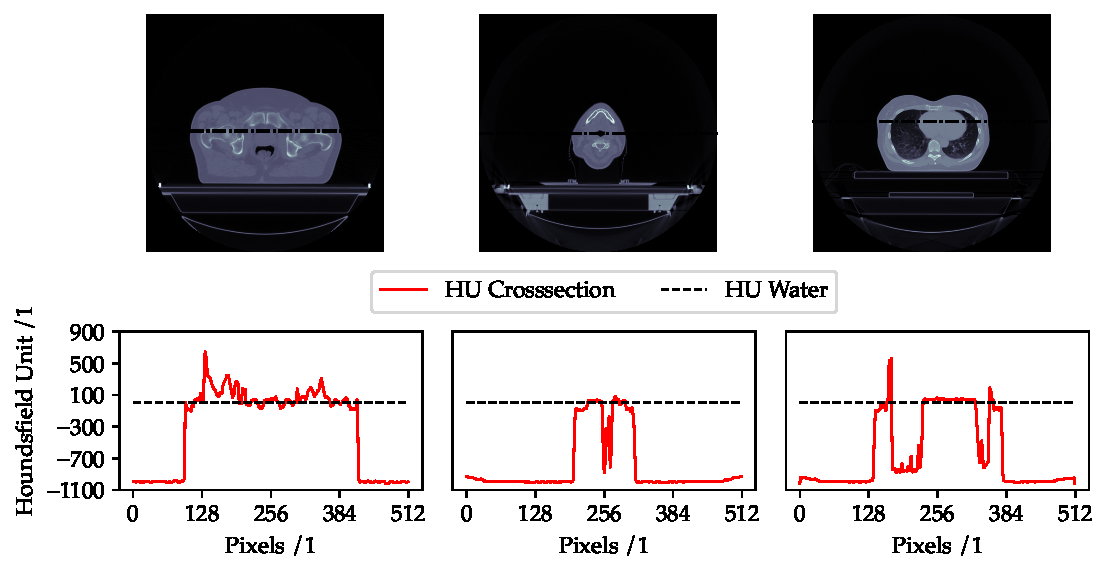
\includegraphics[width=0.9\textwidth]{cross.pdf}
    \caption{
        Top: Image of the isocentric slice from a prostate, H\&N and breast cancer patient respectively. 
        Bottom: Cross section through the patients anatomy at the marked position.
        HU value of water indicated with a dotted line.}\label{fig:crosssection}
\end{figure}

\subsection{Mixed entity training}

The number of patches to convergence was lower for the mixed entity model than for the single entity model, at $5.0 \times 10^7$ compared to $6.7 \times 10^7$ patches.
This suggests that the model learns the important aspects of dose deposition more quickly with the greater diversity of training data than with a relatively homogeneously distributed training data set. 
Model performance and dose prediction accuracy increased for the newly added entities aswell as the \acs{LN} segments aswell as plans. 
Slight decreases in model accuracy regarding single segments of prostate treatment plans are noticed. 
This is most likely due to the increased generalization of the model and the decreased adaption to prostate plans only.
Nevertheless the increased generalization leads to a better perfomance in the mean for the entire prostate plans compared to the prostate-only trained model.
We have observed that the mean single segment prediction accuracies for all entities are smaller than the mean plan prediction accuracies.
As depicted in th lower plot of \autoref{fig:weight_fz_analysis}, the higher weighted segments tend to be predicted better for both models leading to the effect of better predicted plans.\\
Predictions for breast cancer segments are particularly bad for the prostate-only aswell as the mixed-entity trained model. 
Beside the challenging anatomy of air cavities as well as tangential fields only partially hitting the patients body, the internal treatment protocol has changed between training and target dataset. 
Breast cancer treatment plans from the test dataset are significantly higher modulated, with 23.7 ± 5.6 and 83.8 ± 15.3 segments per plan for old and new institutional guidelines respectively. 
This higher modulation results in more smaller segments and more complex \acs{MLC} configurations.
Nevertheless the newly adapted model showed promising results for all tested entities regarding entire plan dose distributions.
As the model needs specific accelerator setting to predict a dose for a specific segment, this model is not usable as a primary dose engine for a radio treatment planning system.
However due to its promising accuracy concernning DVH parameters and its short inference times, it may be promising as an online dose verification or a secondary dose engine after further development.

\subsection{Dose deposition physics}

Water phantoms are used clinically for dose verification and accelerator constancy testing.
Water phantoms are not only the most basic model of a target volume, but dose distributions in them are very well described in literature.
Due to the homogenous density distribution inside the phantom physical processes of dose distribution can be analyzed very well with a water phantom.
We therefore choose a synthetic water phantom to assess the capability of the model to learn the underlying phyisics of the dose deposition process.
Dose curves were resembled by the networks prediction quiet well, dose peaks at the beginning of the phantom were present. 
The exponential dose decrease aswell as the rapid dose drop to the zero level at the end of the phantom has been mapped well qualitatively.
The prostate-only trained model showed particular problems reaching the correct predicted height.
Scaling the curves to the correct maximum, as shown in \autoref{fig:scaled}, gives a more comprehensible picture of the curvature for the prostate-only and mixed entity models.
As depicted the qualitative curvature is closer resembled by the prostate model. 
When comapring different entity crosssections, as shown in \autoref{fig:crosssection}, the prostate density distribution is comparable to the one of a water phantom. 
Therefore it is probable that the model has not learned the underlying pyhsics but predicts the qualitative dose distribution in a water phantom better due to the similarities between the density distribution of the lower abdomen and the one of a water phantom.

\begin{figure}
    \centering
    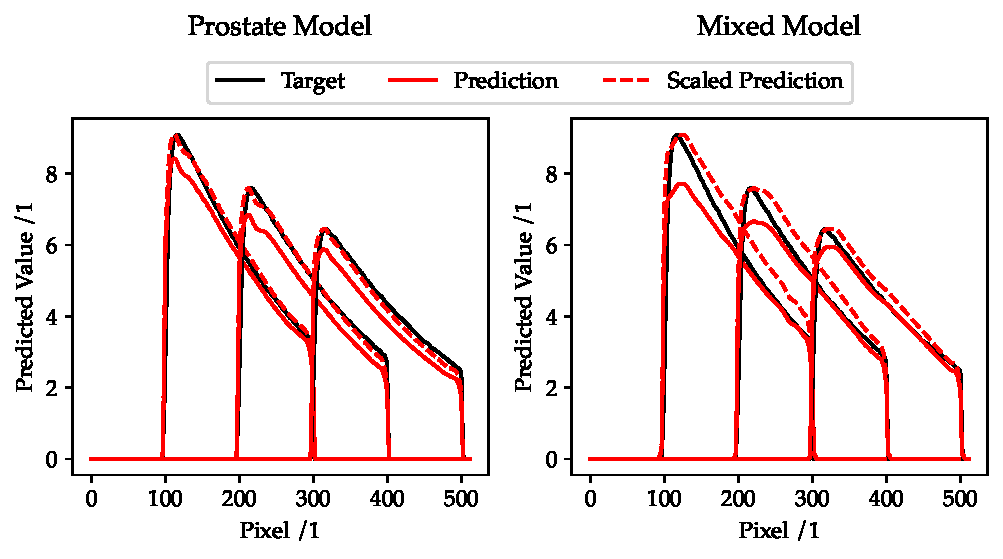
\includegraphics[width=0.9
    \textwidth]{scale.pdf}
    \caption{
        Target, predicted and scaled predicted depth dose curve for water phantom positions at 100, 200 and 300 pixels depth, respectively, from left to right. Left: prostate-only trained model. Right: mixed entity trained model. 
    }\label{fig:scaled}
\end{figure}

Both models have problems with the representation of the dose deposition peak at the beginning of the phantom.
Taking this into account could explain why the dose from the tangential radiation fields represented in \autoref{fig:mamma} is underestimated in the breast cancer plans.
The prediction accuracy of the first 100 pixels of the segment is quite poor, so segments whose radiological path is less than 100 pixels are predicted very poorly.
Cotrary to the first 100 pixels is the dose distribution well resembled by the mixed entity model.
The majority of plans have their target volume and therefore the high dose volume located at higher depths.
As the models prediction of dose curvature at greater depths become more accurate and the gamma passrates only accounts for high dose areas, the gamma passrates increases for target volumes at higher depths.

\subsection{Model improvement}

The here proposed model showed promising results as a first step towards a fast, accurate and robust dose enginge for an online treatment workflow using an MR-Linac. 
We have showed that the genereal concept of a spatial information informed 3D-UNet is applicable for the prediction of dose deposition processes in patients anatomy.
Nevertheless the evaluation of dose prediction accuracy has shown outliers, especially on challenging tasks such as dose distributions in highly heterogenous tissues such as air cavities aswell as very small fields with short radiological paths inside the patients anatomy.  
The network has shown short estmiation times with approximately 3~seconds per segment. 
To improve inference time, investigations towards the expolration of other applicable memory efficient network architectures are needed, aswell as the utilization of a multi GPU prediction process at inference.
In detail analysis of mask impact for every provided mask, as partially done by \citeauthor{kontaxis_deepdose_2020} in \cite{kontaxis_deepdose_2020}, might yield benefitial results for the interpretability of the networks performance as well as its limitations towards a robust and reliable dose prediction. 
As discussed in \autoref{ssec:SET}, we assume that the center beam line distance, might have a negative effects regarding offset segments. \\
We have shown that incorporating more heterogenous training data improves the robustness and the prediction accuracy of the model.
Our training data consisted of patient specific segments combined inside an entire radio treatment plan that was genereated by the treatment planning software. 
This way we had no control over how segments were shaped or oriented.
To achieve desired distributions for fieldsize and gantry angle and to gain control over the segment shapes and the respective iso center, we propose to further increase the training data variability by generating artificial segments.
By using artificial segments, we can control the exact distributions of gantry angles aswell as fieldsizes over the entire training data pool, which might lead to an increased representation of otherwise underpresented segment shapes, sizes and areas of very uncommon iso centers.\\
Data from patients that were previously treated at the MR-linac in our institution is very limited.
We therefore propose to use, in addition to arrtificial segments, the anatomy CTs of not only treated patients at the MR-Linac, but any patient CT\@.
By doing so, we deviate from the small pool of cancer patient CTs from our radiotherapy department and increase the pool to any patient that has taken a CT on any given body region.
This decreases the change of the network overfitting to specific anatomic distribrutions of the given patient anatomy pool and contributes to the robustness and generalization process that is desired to be achieved.
Implementing this approach would suit as a first proof of concept. 
Further data individualization can be achieved by deviating from the patient's anatomy and creating artificial target volumes with heterogeneous areas within the irradiated volume.
The position, shape and density of these created areas inside the target volume, can be choosen based on the desired distribution.\\

Further development could go towards exploring an LSTM approach that provides 2.5-D or 3-D dose distributions in the direction of the irradiation angle, as suggested by \citeauthor{neishabouri_long_2020} in her work on proton dose predictions for heterogeneous tissues~\cite{neishabouri_long_2020}. 
Approching the problem in this manner might lead to networks incorporating of previously seen tissues.
As stated in \autoref{par:radiological_depth} the radiological depth is of crucial importance for the dose deposition processes on the particle path.
Implementing a LSTM would account for the crucial information of prior passed tissues, accounting for the vanishing gradient problem. 
Further information incorporated into the model input, such as a vector mask to indicate the Lorentz force acting on the secondary particles, could increase in a more accurate dose deposition prediction.\\

In contrast to \citeauthor{kontaxis_deepdose_2020}~\cite{kontaxis_deepdose_2020} we decreased the voxel size of the target volume in the coronal and sagital plane. 
Longer predicion times of 3~seconds per segment were the result.

The model shows short prediction times, with 3~seconds per segment, which is a first step towards an online plan adaption process involving the MR-linac.





%- erweiterung der arbeit:
%- was können wir machen um das netwerk vielleicht zu verbessern
%- neue masken? investigation needed
%- neue netzwerk architektur
%- erweiterung des netzwerkes um den strahl entlang der strahlrichtung zu verfolgen und somit effekte aus vorherigen schichten besser zu beachten
%- änderung der trainings daten
%- keine wirklichen segmente mehr
%- also atifizielle formen, größen, isocentren und auch bestrahlungswinkel
%- keine wirklich bestrahlten patienten mehr sondern einfach irgendwelche CTs von verschiedenen Körperregionen
%- garkeine wirklichen patientendaten mehr -> könnte dazu führen dass das netzwerk so gut generalisiert, dass es wirklich egal ist was man ihm gibt
%- so erreicht mehr variabilität, hat mehr kontrolle über verteilungen von winkeln und auch feldgrößen und formen

- ausblick wenn diese dosisberechnung robust und auch schnell ist kann sie in der workflow am mr linac so eingebunden werde, dass man keine normale dosisberechnung mehr brauch und wir somit der adaptive bestrahlung einen schritt näher gekommen sind. 
- dafür müsste die interpretiertbarkeit von ML in medizin erhöht werden, sonst keine Information darüber ob jetzt ein segment gut oder schlecht predichtet wird.
- approach mit unsicherheit, auf paper verweisen. Uncertainty quantification

% - etwas auf die physik eingehen, zeigen, dass das netwerk bei einem einfachen 10x10 feld eine gute vorhersage treffen kann. woher das peak problem kommt keine ahnung? auch problem mit dem zu schnellen abflachen der schultern keine ahnung vllt nochmal besprechen. prostata model ist irgendwie nicht fähig die korrekte höhe anfangs zu finden, was aber egal ist weil der dosisaufbau aller segmente eigentlich eher in der tiefe passiert und das dann bei dem gamma nicht so ins gewicht fällt. evtl das problem bei den ganzen kleinen mamma segmenten, da da ja die dosis besonders bei den tangentialen kleinen feldern eher am anfang interesant ist. 
% - zeigen, dass das model anscheinend kein problem mit unterscheidlichen auflösungen in verschiedene raumrichtungen hat. Model ist dann denkbar erweiterbar auf verschiedene grid spacings, wenn man das möchte und es sinnvoll ist.

\vspace*{50pt}

%- Erstes Model bietet sehr gute Ergebnisse wenn man es auf den benutzen Daten auch testet.
%- Gamma passrate wie auch das DVH zeigen sehr gute Übereinstimmung zwischen original und prediction. 
%- Klinisch akzeptabel??
-> klinisch primär nicht nutzbar, wegen interpretierbarkeit und nicht gut genug, online dose verification oder second dose, phase 1 für planoptimierung anstatt peniclbeam, peniclbeam stellt mr feld nicth dar und auch probleme bei dichtegradienten 

%- zeigen, dass die prediction unabhängig von der feldform oder einstrahlrichtung ist.
%- Prediction time drauf eingehen, also 3 sekunden vs 4 stunden, führt in Richtung online adaption
%- Kontrast zu DeepDose vllt hervorheben bezüglich Winkel, und voxelgröße -> wichtig
%- bezug nehmen darauf das weitere entitäten die sich in form größe und position der felder sehr unterscheiden nicht mehr so gut funktionieren. -> selbst bei entitäten unterschiede, je nach planungsform, mamma unterschiede, conventionelle mamam zu apbi 
- bezug nehmen auf die Werte, bzw auch ein paar DVH kriterien mal ausfzeigen. (hab keine werte in Gy, brauch ich das überhaupt?) -> brauchen wir
%- besondere ausreißer hervorheben (Mamma), kurz darauf eingehen was sich denn eigentlich da unterscheidet
%- warum vermuten wir dass es nicht so gut geht
%- was ändert sich eigentlich zb bei nem Mamma plan bzw nem HNO Plan eingehen auf ändernde Feldgröße und Feldformen und SSD und auch Verteilung der Anatomie generell, HU units etc. siehe grafik crossection. 

%- dann kurz darauf eingehen, dass das Training mit dem neuen Netzwerk doch irgendwie schneller ging und weniger patches benötigt worden um zu konvergieren
%- zeigen, sagen dass wir so in das Training weitere SSD, Isozentrum und MLC shapes eingebunden haben und wir uns davon versprechen, dass das netzwerk eher generealisiert
- Dann darauf evtl eingehen, dass Feldgrößen von 53 mm feldlänge maximal in 32 Pixeln abgebildet werden kann, das ist auch der punkt ab dem besonders bei dem prostata model aber auch bei dem mixed model die performance abnimmt. 

% - auf Ergebnisse eingehen, dass wir auf jeden fall einen signifikanen anstieg der performance beobachten konnten auf mixed und lymph und einen significanten slight decrease wenns es um die einzelsegmente geht bei prostata (abweichung im mean) aber bei den plänen sieht die performance dann wieder besser aus. sagen dass segmente generell schlechter sind, was aber auch daran dann liegt, dass kleine felder genrell schlechter performen aber bei so einer auswertung gleich gewichtet werden obwohl sie ja zum gesamt plan viel weniger contributen

%- darauf eignehen, dass sich das protokoll bei der erstellung von Mamma fällen zwischen training und test daten geändert hat.
%- Anschauen welche Segmente denn so schlecht bei Mamma performen, es sind alles kleine segmente,zb: mt0\_55 mt0\_6 mt2\_16 mt0\_57 mt1\_58 mt4\_58 mt4\_74 mt2\_17 mt0\_5 mt0\_43 mit den fz: 2.333 2.5605 5.329 3.8893 3.4712 2.819 2.0261 5.4375 2.8592 6.509 und den gammas: 1.8935 2.3627 3.0733 3.2233 5.765 7.33 9.26 14.9003 15.81 16.93
%- besonders tangentiale kleine felder sind extrem schwierig, man kann sehen, dass der algorithmus prinzipiell unterschätzt als überschätzt. vllt hiern noch ne analyse machen?! zu zeit aufwendig evtl.

- eingehen auf die grafik mit den feldgrößen und die verteilung der feldgrrößen, evlt. ins training evtl mehr kleine einbauen, damit diese besser werden. oder eher die felder berücksichtigen die mehr contribution zu einem plan haben (große?). normal verteilt? dann verteilung  der winkel beachten?




